\documentclass[12pt]{article}

% Layout.
\usepackage[top=1in, bottom=0.75in, left=1in, right=1in, headheight=1in, headsep=6pt]{geometry}

% Fonts.
\usepackage{mathptmx}
\usepackage[scaled=0.86]{helvet}
\renewcommand{\emph}[1]{\textsf{\textbf{#1}}}

% TiKZ.
\usepackage{tikz, pgfplots}

\usetikzlibrary{calc,trees,positioning,arrows,fit,shapes,through, backgrounds}
\usetikzlibrary{patterns}

\usetikzlibrary{decorations.markings}
\usetikzlibrary{arrows}

\usepackage{pgfplots}


% Misc packages.
\usepackage{amsmath,amssymb,latexsym}
\usepackage{graphicx}
\usepackage{array}
\usepackage{xcolor}
\usepackage{multicol}
\usepackage{fancyhdr}
\pagestyle{fancy}


% Misc.
\renewcommand{\d}{\displaystyle}
\newcommand{\ds}{\displaystyle}
\newcommand{\ul}[1]{\underline{#1}}
\def\bc{\begin{center}}
\def\ec{\end{center}}
\def\be{\begin{enumerate}}
\def\ee{\end{enumerate}}

\newcommand{\ans}[1][1in]{\rule{#1}{.5pt}}


\lhead{Math F113X: Quiz 5}
\rhead{Spring 2026}

\begin{document}

\vspace{1cm}
\strut

\noindent \textbf{Name:} \hrulefill \quad  score:\ans[1cm] \ / 10 \\


\noindent There are 10 points possible on this quiz. No aids (book, notes, etc.)
are permitted. You may use a calculator.  {\bf Show all work and supporting calculations for full credit. Explain how you get your answers.}



\be

\item (3 points) Answer questions about the graph below. \\

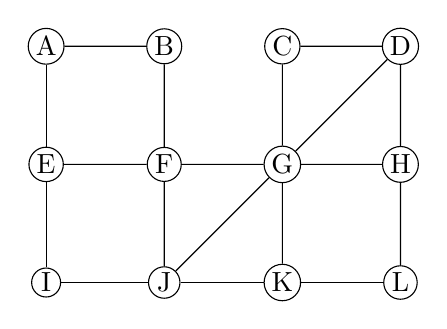
\begin{tikzpicture}[baseline=(current bounding box.center),scale=1.5]
\tikzstyle{vertex}=[circle, draw, inner sep=1pt]
\tikzstyle{every node} = [vertex];
\node (A) at (0,2) {A};
\node (B) at (1,2) {B};
\node (C) at (2,2) {C};
\node (D) at (3,2) {D};;
\node (E) at (0,1) {E};
\node (F) at (1,1){F};
\node (G) at (2,1){G};
\node (H) at (3,1){H};
\node (I) at (0,0) {I};
\node (J) at (1,0) {J};
\node (K) at (2,0) {K};
\node (L) at (3,0) {L};
\foreach \i/\j in {A/B,C/D,E/F,F/G,G/H,I/J,J/K,K/L,A/E,B/F,G/C,D/G,E/I,F/J,G/J,G/K,H/L,D/H}{\draw (\i) -- (\j);}
\end{tikzpicture}
	\begin{enumerate}
	\item \textbf{Circle} or \textbf{shade} all vertices of odd degree.
	\item Determine if the graph has an Euler circuit. Justify your answer.

	\end{enumerate}
\vspace{1in}


\item (3 points) Eulerize the graph below \textbf{using as few edge duplications as possible.} \\


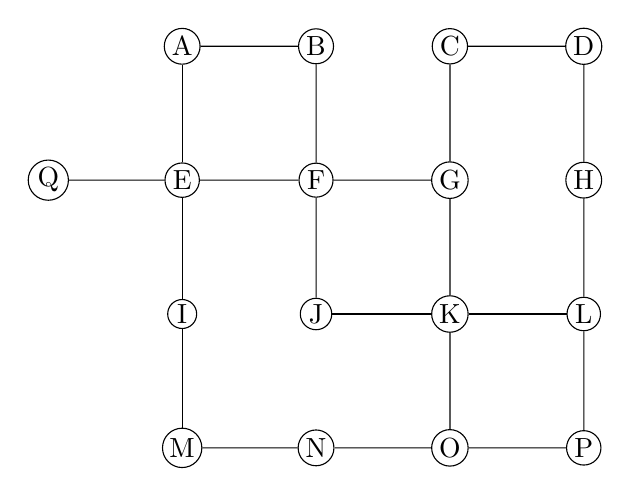
\begin{tikzpicture}[baseline=(current bounding box.center),lbl/.style={inner sep = 2pt, fill = white}, scale = 1.7]
\tikzstyle{vertex}=[circle, draw, inner sep=1pt]
\tikzstyle{every node} = [vertex];
\node (a) at (0,2) {A};
\node (b) at (1,2) {B};
\node (c) at (2,2) {C};
\node (d) at (3,2) {D};
\node (e) at (0,1) {E};
\node (f) at (1,1){F};
\node (g) at (2,1){G};
\node (h) at (3,1){H};
\node (i) at (0,0) {I};
\node (j) at (1,0) {J};
\node (k) at (2,0) {K};
\node (l) at (3,0) {L};
\node (m) at (0,-1) {M};
\node (n) at (1,-1) {N};
\node (o) at (2,-1) {O};
\node (p) at (3,-1) {P};
\node (q) at (-1,1) {Q};
\foreach \i/\j in {q/e,a/b,c/d,e/f,f/g,g/k,j/k,k/l,m/n,n/o,o/p,a/e,b/f,c/g,d/h,e/i,i/m,f/j,h/l,l/p,k/o}{\draw (\i) -- (\j);}
\end{tikzpicture}
\vfill
\newpage
\item (2 points) Find a Euler \emph{path} in the graph, $G$,  below. Indicate your path by drawing arrows on the edges and numbering the edges.  Label the starting and ending vertices. (There is a copy of the graph as scratch if needed. \textbf{Clearly indicate which graph you want graded.})\\

\vspace{.5in}


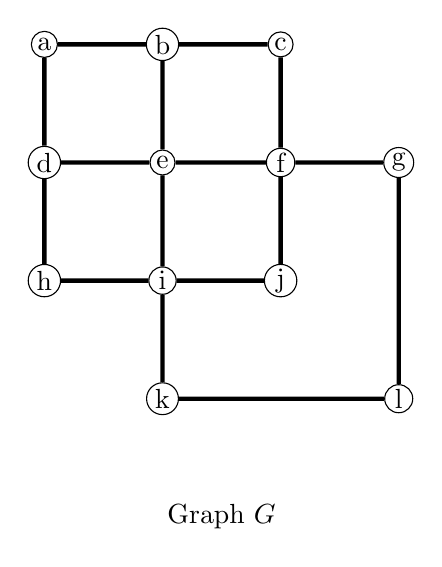
\begin{tikzpicture}[scale=1.5]
\node at (1.5,-1){Graph $G$};
\tikzstyle{vertex}=[circle, draw, inner sep=1pt]
\tikzstyle{every node} = [vertex];
\node (a) at (0,3) {a};
\node (b) at (1,3) {b};
\node (c) at (2,3) {c};
\node (d) at (0,2) {d};
\node (e) at (1,2) {e};
\node (f) at (2,2) {f};
\node (g) at (3,2) {g};
\node (h) at (0,1) {h};
\node (i) at (1,1) {i};
\node (j) at (2,1) {j};
\node (k) at (1,0) {k};
\node (l) at (3,0) {l};
\draw[ultra thick] (d) -- (a)--(b)--(c)--(f)--(g)--(l)--(k)--(i)--(j)--(f)--(e)--(i)--(h)--(d)--(e)--(b);
\end{tikzpicture}
\hfill
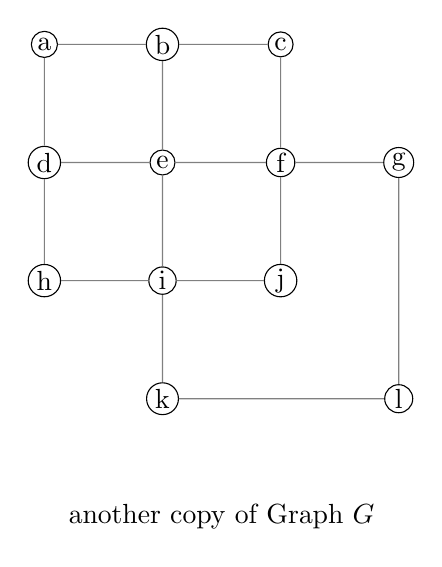
\begin{tikzpicture}[scale=1.5]
\node at (1.5,-1){another copy of Graph $G$};
\tikzstyle{vertex}=[circle, draw, inner sep=1pt]
\tikzstyle{every node} = [vertex];
\node (a) at (0,3) {a};
\node (b) at (1,3) {b};
\node (c) at (2,3) {c};
\node (d) at (0,2) {d};
\node (e) at (1,2) {e};
\node (f) at (2,2) {f};
\node (g) at (3,2) {g};
\node (h) at (0,1) {h};
\node (i) at (1,1) {i};
\node (j) at (2,1) {j};
\node (k) at (1,0) {k};
\node (l) at (3,0) {l};
\draw[thin, gray] (d) -- (a)--(b)--(c)--(f)--(g)--(l)--(k)--(i)--(j)--(f)--(e)--(i)--(h)--(d)--(e)--(b);
\end{tikzpicture}
\vfill
\item (2 points) Find a Hamiltonian circuit of minimum weight in the graph below. Several other copies of the graph provided. \\


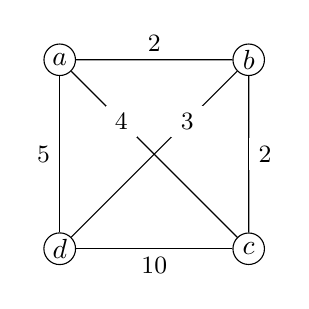
\begin{tikzpicture}[scale=1.2,
  every node/.style={circle, draw, fill=white, minimum size=4mm,inner sep=1pt},
  every edge/.style={draw},
  lbl/.style={rectangle, draw=none, fill=white, inner sep=1pt, font=\small}
]
% Vertices at corners of a square
\node (a) at (0,2) {$a$};
\node (b) at (2,2) {$b$};
\node (c) at (2,0) {$c$};
\node (d) at (0,0) {$d$};
% Edges with weights
\draw (a) -- node[lbl, above] {2} (b);
\draw (a) -- node[lbl, left]  {5} (d);
\draw (a) -- node[lbl, above left, pos=0.4] {4} (c);
\draw (b) -- node[lbl, right] {2} (c);
\draw (b) -- node[lbl, above right, pos=0.4] {3} (d);
\draw (c) -- node[lbl, below] {10} (d);
\end{tikzpicture}
\hfill
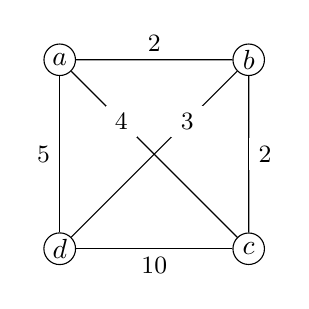
\begin{tikzpicture}[scale=1.2,
  every node/.style={circle, draw, fill=white, minimum size=4mm,inner sep=1pt},
  every edge/.style={draw},
  lbl/.style={rectangle, draw=none, fill=white, inner sep=1pt, font=\small}
]

% Vertices at corners of a square
\node (a) at (0,2) {$a$};
\node (b) at (2,2) {$b$};
\node (c) at (2,0) {$c$};
\node (d) at (0,0) {$d$};

% Edges with weights
\draw (a) -- node[lbl, above] {2} (b);
\draw (a) -- node[lbl, left]  {5} (d);
\draw (a) -- node[lbl, above left, pos=0.4] {4} (c);
\draw (b) -- node[lbl, right] {2} (c);
\draw (b) -- node[lbl, above right, pos=0.4] {3} (d);
\draw (c) -- node[lbl, below] {10} (d);

\end{tikzpicture}
\hfill
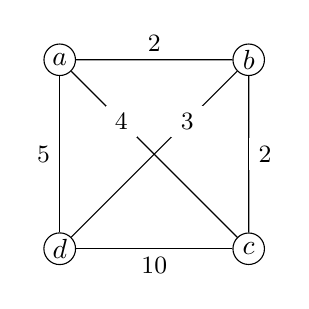
\begin{tikzpicture}[scale=1.2,
  every node/.style={circle, draw, fill=white, minimum size=4mm,inner sep=1pt},
  every edge/.style={draw},
  lbl/.style={rectangle, draw=none, fill=white, inner sep=1pt, font=\small}
]

% Vertices at corners of a square
\node (a) at (0,2) {$a$};
\node (b) at (2,2) {$b$};
\node (c) at (2,0) {$c$};
\node (d) at (0,0) {$d$};

% Edges with weights
\draw (a) -- node[lbl, above] {2} (b);
\draw (a) -- node[lbl, left]  {5} (d);
\draw (a) -- node[lbl, above left, pos=0.4] {4} (c);
\draw (b) -- node[lbl, right] {2} (c);
\draw (b) -- node[lbl, above right, pos=0.4] {3} (d);
\draw (c) -- node[lbl, below] {10} (d);

\end{tikzpicture}
\hfill 
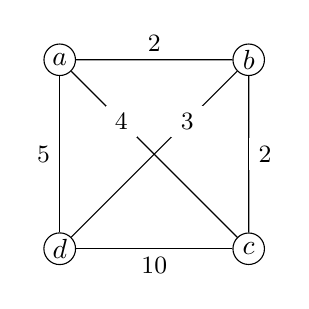
\begin{tikzpicture}[scale=1.2,
  every node/.style={circle, draw, fill=white, minimum size=4mm,inner sep=1pt},
  every edge/.style={draw},
  lbl/.style={rectangle, draw=none, fill=white, inner sep=1pt, font=\small}
]

% Vertices at corners of a square
\node (a) at (0,2) {$a$};
\node (b) at (2,2) {$b$};
\node (c) at (2,0) {$c$};
\node (d) at (0,0) {$d$};

% Edges with weights
\draw (a) -- node[lbl, above] {2} (b);
\draw (a) -- node[lbl, left]  {5} (d);
\draw (a) -- node[lbl, above left, pos=0.4] {4} (c);
\draw (b) -- node[lbl, right] {2} (c);
\draw (b) -- node[lbl, above right, pos=0.4] {3} (d);
\draw (c) -- node[lbl, below] {10} (d);

\end{tikzpicture}

\vfill
vertices of the Hamiltonian circuit: \underline{\hspace{1.5in}} \hfill weight: \underline{\hspace{1in}}
\vfill 
 \ee
\end{document}